\documentclass[11pt]{article}

\usepackage[margin=1in]{geometry}
\usepackage{amsmath,amssymb,bm}
\usepackage{graphicx}
\usepackage{booktabs}
\usepackage{array}
\usepackage{float}
\usepackage{xcolor}
\usepackage{hyperref}

% Trained-run outputs (hw3_results) take priority over the original hw3-update copies.
\graphicspath{{./}}

% Homework prompt, set off from the writeup that follows.
\newenvironment{question}{%
  \par\addvspace{0.8em}%
  \begin{quote}\small
  \noindent\textbf{Question.}\enspace\ignorespaces
}{%
  \end{quote}%
  \par\nopagebreak
  \noindent\textbf{Response.}\par\nopagebreak\smallskip
}

% Placeholder for answers still to be written. Grep for \fillin before submitting.
\newcommand{\fillin}[1]{\par\noindent{\color{red}\textbf{[TODO]} #1}\par}

\newcommand{\KL}{D_{\mathrm{KL}}}
\newcommand{\E}{\mathbb{E}}
\newcommand{\R}{\mathbb{R}}
\newcommand{\ind}{\mathbf{1}}

\title{ECE 6257-GDL, Fall 2026\\Problem Set 3 Solutions}
\author{Michael Incorvaia}
\date{}

\begin{document}
\maketitle
\tableofcontents
\newpage

%%%%%%%%%%%%%%%%%%%%%%%%%%%%%%%%%%%%%%%%%%%%%%%%%%%%%%%%%%%%%%%%%%%%%%%%
\section{Problem 1: GANs on MNIST (40 points)}
%%%%%%%%%%%%%%%%%%%%%%%%%%%%%%%%%%%%%%%%%%%%%%%%%%%%%%%%%%%%%%%%%%%%%%%%
% Body below is gan-mnist-writeup.tex (hw3/hw3-update/), sections demoted one
% level, with the four sample grids added as figures.

\begin{question}
You will implement a Generative Adversarial Network model and evaluate it under different conditions, using the notebook \texttt{gan-mnist.ipynb}.
\begin{enumerate}
  \item[(a)] Part 1: Libraries and utility functions. Why do you think it is convenient to normalize the images to the range \([-1,1]\) instead of \([0,1]\)?
  (Bonus) How does the minimax game defined by the objective function of a GAN relate to minimizing the Jensen--Shannon divergence between the training data distribution and the samples obtained from the generator? (Bonus) Why is maximizing the probability of the discriminator making the INCORRECT choice the most practical way to update the generator?
  \item[(b)] Part 2: Vanilla GAN. Implement the noise sampling function as well as the generator and discriminator networks.
  \item[(c)] Part 3: GAN Loss. Implement the necessary losses for both networks.
  \item[(d)] Part 4: Training Function. Implement the optimizer construction, review and run the training loop cells. How do the generated samples look?
  \item[(e)] Part 5: Least Squares GAN. Implement the Least-Squares loss function and evaluate. How do the resulting generated samples compare to those produced by the Vanilla GAN? Why do you think this is the case?
  \item[(f)] Part 6: Deeply Convolutional GANs. Implement the generator and discriminator architectures and evaluate the resulting model. How do the generated samples compare to the two previous configurations? Why does adding convolutional layers have this effect?
  \item[(g)] Part 7: Compare generated images. Evaluate the generated samples from the three previous models against the real MNIST images. Can you distinguish the original from the fake ones in all three cases? Do you think an equilibrium exists where the generator wins, i.e.\ the discriminator ends up unable to distinguish the two distributions on finite samples? Explain why you believe this would or would not be possible.
\end{enumerate}
\end{question}

\subsection{Part 1: Libraries and Utility Functions}

The notebook defines the GAN as the minimax game
\begin{equation}
  \min_G \max_D \;
  \mathbb{E}_{x \sim p_{\mathrm{data}}}\!\left[\log D(x)\right]
  + \mathbb{E}_{z \sim p(z)}\!\left[\log \bigl(1 - D(G(z))\bigr)\right],
  \label{eq:minimax}
\end{equation}
and then replaces the generator step with
\begin{equation}
  \max_G \; \mathbb{E}_{z \sim p(z)}\!\left[\log D(G(z))\right].
  \label{eq:nonsat}
\end{equation}
\texttt{preprocess\_img} maps real images from \([0,1]\) to \([-1,1]\) by \(x \mapsto 2x-1\), and \texttt{deprocess\_img} maps them back for display.

\subsubsection{Normalization to \([-1,1]\)}

Scaling to \([-1,1]\) matches the generator's final \(\tanh\), whose outputs lie in \((-1,1)\). Real and generated images then share one scale, so the discriminator compares like with like and every real pixel value is one the generator can actually produce. The interval is also symmetric about zero, which keeps the inputs to both networks roughly zero-mean, and it matches the range of the latent noise.

\subsubsection{Minimax training and Jensen--Shannon divergence}

For a fixed generator, the discriminator that maximizes~\eqref{eq:minimax} is
\begin{equation}
  D_G^*(x) = \frac{p_{\mathrm{data}}(x)}{p_{\mathrm{data}}(x) + p_g(x)}.
\end{equation}
Substituting \(D_G^*\) back in gives
\begin{align}
  C(G)
  &= -\log 4
    + \mathrm{KL}\!\left(p_{\mathrm{data}} \middle\| \frac{p_{\mathrm{data}}+p_g}{2}\right)
    + \mathrm{KL}\!\left(p_g \middle\| \frac{p_{\mathrm{data}}+p_g}{2}\right) \nonumber \\
  &= -\log 4 + 2\,\mathrm{JSD}(p_{\mathrm{data}} \| p_g).
  \label{eq:jsd}
\end{align}
The inner maximization turns the game into a constant plus twice the Jensen--Shannon divergence between the data and generator distributions, so minimizing over \(G\) minimizes that divergence. The minimum, \(-\log 4\), is reached only when \(p_g = p_{\mathrm{data}}\), where \(D_G^*(x) = 1/2\) everywhere.

\subsubsection{Generator update}

Early in training the generator is weak and \(D(G(z)) \approx 0\). With \(D = \sigma(s)\) for a logit \(s\), the minimax generator term \(\log(1-D(G(z)))\) has gradient \(-D(G(z))\) with respect to \(s\), which goes to zero there, so the generator gets almost no signal.

The non-saturating update~\eqref{eq:nonsat} instead minimizes \(-\mathbb{E}_z[\log D(G(z))]\), whose gradient with respect to \(s\) is \(-(1 - D(G(z)))\). That is largest exactly when \(D(G(z))\) is near \(0\). It maximizes the probability that the discriminator is wrong on generated data, keeps the same fixed point (\(p_g = p_{\mathrm{data}}\), \(D = 1/2\)), and gives much larger gradients early on. The discriminator still trains on~\eqref{eq:minimax}.

\subsection{Part 2: Vanilla GAN}

\subsubsection{Noise sampling}

\texttt{sample\_noise(batch\_size, dim)} draws \texttt{torch.rand} of shape \((\texttt{batch\_size}, \texttt{dim})\), uniform on \([0,1]\), and maps \(u \mapsto 2u-1\). The result is the uniform prior on \([-1,1]\).

\subsubsection{Discriminator}

A fully connected classifier with biases and LeakyReLU slope \(0.01\):
\begin{center}
\begin{tabular}{lll}
\toprule
Layer & Shape & Activation \\
\midrule
Flatten & image \(\to\) \(784\) & none \\
Linear & \(784 \to 256\) & LeakyReLU(\(0.01\)) \\
Linear & \(256 \to 256\) & LeakyReLU(\(0.01\)) \\
Linear & \(256 \to 1\) & none \\
\bottomrule
\end{tabular}
\end{center}
It outputs one logit per image, shape \([\texttt{batch\_size}, 1]\). There is no sigmoid, so the loss can use a numerically stable cross-entropy on logits. The network has \(267{,}009\) parameters.

\subsubsection{Generator}

\begin{center}
\begin{tabular}{lll}
\toprule
Layer & Shape & Activation \\
\midrule
Linear & \(\texttt{noise\_dim} \to 1024\) & ReLU \\
Linear & \(1024 \to 1024\) & ReLU \\
Linear & \(1024 \to 784\) & \(\tanh\) \\
\bottomrule
\end{tabular}
\end{center}
The final \(\tanh\) puts every pixel in \((-1,1)\), the range of the preprocessed real images. With \(\texttt{noise\_dim} = 4\), as in the notebook's parameter check, the network has \(1{,}858{,}320\) parameters; training uses \(\texttt{NOISE\_DIM} = 96\).

\subsection{Part 3: GAN Loss}

Both losses are minibatch means of the provided stable binary cross-entropy on logits,
\[
  bce(s, y) = -y \log \sigma(s) - (1-y)\log\bigl(1-\sigma(s)\bigr),
\]
with real targets \(1\) and fake targets \(0\). Scores of shape \([N, 1]\) are flattened to length \(N\) so they line up with the labels, which are cast to the scores' device with \texttt{.type(dtype)}.

\subsubsection{Discriminator}

\[
  \ell_D
  = -\mathbb{E}_{x \sim p_{\mathrm{data}}}\!\left[\log D(x)\right]
  - \mathbb{E}_{z \sim p(z)}\!\left[\log \bigl(1 - D(G(z))\bigr)\right].
\]
In code this is \texttt{loss\_real + loss\_fake}: real logits against ones plus fake logits against zeros. Since \texttt{bce\_loss} returns a mean, the sum matches the two expectations. Minimizing it raises \(D(x)\) on real images and lowers \(D(G(z))\) on fakes.

\subsubsection{Generator}

The non-saturating objective from Part~1, written for minimization:
\[
  \ell_G = -\mathbb{E}_{z \sim p(z)}\!\left[\log D(G(z))\right].
\]
It is the cross-entropy between fake logits and ones, which pushes \(D(G(z))\) toward \(1\).

\subsection{Part 4: Training}

\subsubsection{Optimizer}

\texttt{get\_optimizer} returns Adam with learning rate \(10^{-3}\) and betas \((0.5, 0.999)\), used for every network in the notebook. \(\beta_1 = 0.5\) is the usual GAN choice: a shorter gradient memory suits a discriminator that keeps moving.

\subsubsection{Training loop}

The loop is provided. Each epoch runs the \(390\) full minibatches of \(128\) from the \(50{,}000\) training images (the incomplete last batch is skipped), for \(10\) epochs. Each iteration takes one discriminator step, then one generator step. Real images are scaled by \(2(x - 1/2)\), the same map as \texttt{preprocess\_img}. The discriminator step detaches the generated images, so only \(D\) is updated. The generator step draws fresh noise and scores the fakes with the updated \(D\); the gradients this leaves on \(D\) are cleared by the next iteration's \texttt{zero\_grad}. Every \(250\) iterations a fixed noise batch, drawn once at the start, is passed through \(G\) and saved to \texttt{v\_gan/image\_*.png}, so the same latent codes can be followed through training.

\subsubsection{Generated samples}

At iteration \(0\) every tile is gray pixel noise. By iteration \(250\) the mass has collapsed into bright, fuzzy blobs on a still-gray background, most with the same rough 8-like shape. By iteration \(1000\) the backgrounds are dark and the blobs have become soft digits: nines, sevens, zeros, and ones are recognizable, with speckled edges. At iterations \(3000\) and \(3750\) about half of the fixed seeds are clearly a digit (\(1\), \(4\), \(6\), \(7\)); the rest are broken or noisy, and speckle remains around most strokes. The discriminator loss stays near \(1.0\)--\(1.4\), around the equilibrium value \(2\log 2 \approx 1.39\), and the generator loss settles near \(0.8\)--\(1.1\) after an early spike. The samples cover a spread of digit classes rather than a single mode.

\begin{figure}[H]
  \centering
  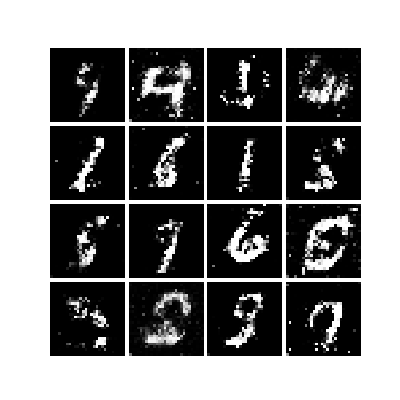
\includegraphics[width=0.55\linewidth]{v_gan/image_015.png}
  \caption{Vanilla GAN, this run's fixed latent codes at iteration 3750.}
  \label{fig:vgan}
\end{figure}

\subsection{Part 5: Least Squares GAN}

The networks and training loop stay the same; only the losses change, to equation~(9) of Mao et al.:
\begin{align}
  \ell_D
  &= \tfrac12 \mathbb{E}_{x \sim p_{\mathrm{data}}}\!\left[\bigl(D(x)-1\bigr)^2\right]
   + \tfrac12 \mathbb{E}_{z \sim p(z)}\!\left[\bigl(D(G(z))\bigr)^2\right], \\
  \ell_G
  &= \tfrac12 \mathbb{E}_{z \sim p(z)}\!\left[\bigl(D(G(z))-1\bigr)^2\right].
\end{align}
Each expectation is a minibatch mean of the raw scores. Against \texttt{gan-checks.npz} the errors are \(1.53\times 10^{-8}\) for the discriminator and \(2.78\times 10^{-9}\) for the generator, both under the \(10^{-7}\) tolerance.

\subsubsection{Comparison with the vanilla GAN}

At iteration \(1000\) the LS samples are still clusters of salt-and-pepper pixels, behind the vanilla grid at the same point. By iterations \(3000\) and \(3750\) most fixed seeds are a recognizable digit (\(5\), \(3\), \(9\), \(1\), \(4\), \(6\), \(7\)), with thicker and more complete strokes than the vanilla samples, where only about half are clearly digits. The gain is modest in this run: the speckle around the strokes is about as heavy as in the vanilla grid, a few seeds are still blobs, and the \(4\) repeats several times.

The more complete strokes come from the loss. The vanilla generator's cross-entropy saturates once a fake is on the real side of the decision boundary, so there is little gradient left to fix speckle or broken strokes. The LS generator loss has gradient proportional to \(D(G(z))-1\), which stays large until the score actually reaches \(1\), so fakes that already fool the classifier are still pulled toward the real data. With labels satisfying \(b-c=1\) and \(b-a=2\), Mao et al.\ show that the LS objective minimizes a Pearson \(\chi^2\) divergence. The \(0/1\) labels used here do not meet that condition, but the gradient argument still holds.

\begin{figure}[H]
  \centering
  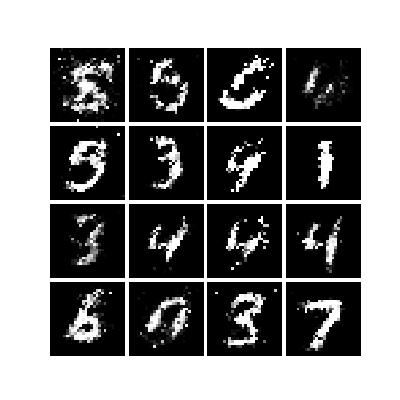
\includegraphics[width=0.55\linewidth]{ls_gan/image_015.png}
  \caption{LSGAN, this run's fixed latent codes at iteration 3750.}
  \label{fig:lsgan}
\end{figure}

\subsection{Part 6: Deep Convolutional GAN}

The loss is back to binary cross-entropy; the networks change. The discriminator unflattens to \(1\times 28\times 28\), then applies conv \(1\to 32\) (\(5\times 5\)), LeakyReLU(\(0.01\)), \(2\times 2\) max-pool, conv \(32\to 64\) (\(5\times 5\)), LeakyReLU, max-pool, flatten, linear \(1024\to 1024\), LeakyReLU, and linear \(1024\to 1\). It has \(1{,}102{,}721\) parameters and outputs shape \([128, 1]\).

The generator follows the InfoGAN layout: linear to \(1024\), ReLU, batch norm; linear to \(128\cdot 7\cdot 7\), ReLU, batch norm; reshape to \(128\times 7\times 7\); then two transposed convolutions (\(4\times 4\), stride \(2\), padding \(1\)) up to \(64\times 14\times 14\) and \(1\times 28\times 28\), with ReLU and batch norm between them and \(\tanh\) at the end. A final flatten returns a \(784\)-vector for the existing training loop. With \(\texttt{noise\_dim}=4\) it has \(6{,}580{,}801\) parameters. Xavier initialization is applied to every linear and transposed-convolution weight in both networks before training.

\subsubsection{Comparison with the fully connected GANs}

Iteration \(0\) is noise. By iteration \(1000\) the fixed seeds are already clean digits on a black background, ahead of where either fully connected model was at iteration \(3750\). At iteration \(3750\) the strokes are smooth and the backgrounds clean: \(1, 3, 7, 9, 8, 5, 8, 3, 1, 1, 5, 0, 9, 6, 7, 3\). A few tiles are slightly soft and the \(6\) is a bit malformed, but there is almost none of the salt-and-pepper noise in the vanilla and LS grids.

Convolution is the reason. A fully connected generator treats the \(784\) pixels as one vector, so nothing in its wiring says strokes are local or that the same edge can appear anywhere; the samples show that as speckle and broken contours. A convolutional discriminator looks at local patches with shared filters, so it judges stroke shape rather than a bag of pixels. The transposed convolutions build the image by upsampling a \(7\times 7\) spatial code, so neighboring pixels are produced together, and batch norm keeps the deeper generator stable. The result is coherent strokes much earlier in training.

The losses are less flattering than the images. Over the last \(1000\) iterations the discriminator loss sits near \(1.0\)--\(1.1\) and the generator loss near \(0.9\)--\(1.3\), on either side of the chance-level pair \(2\log 2 \approx 1.39\) and \(\log 2 \approx 0.69\), so the discriminator still separates real from fake better than chance.

\begin{figure}[H]
  \centering
  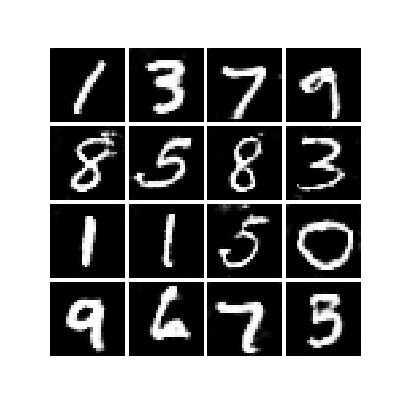
\includegraphics[width=0.55\linewidth]{dc_gan/image_015.png}
  \caption{DCGAN, this run's fixed latent codes at iteration 3750.}
  \label{fig:dcgan}
\end{figure}

\subsection{Part 7: Comparison with real MNIST}

Stacked against real digits, the three generators separate cleanly. Vanilla samples are easy to pick out: broken strokes, speckled backgrounds, and only about half are sharp digits. LS samples are only slightly harder; most are recognizable, but the strokes stay gritty and speckled. DCGAN samples are the close call, and many would pass as MNIST on their own. In a grid of \(50\) fakes over \(50\) reals (Figure~\ref{fig:realfake}), the real half is slightly crisper and the fake half still has the occasional stray pixel, soft edge, or slightly wrong stroke. That is enough to tell the two blocks apart, but not to label every single DCGAN image with confidence.

\begin{figure}[H]
  \centering
  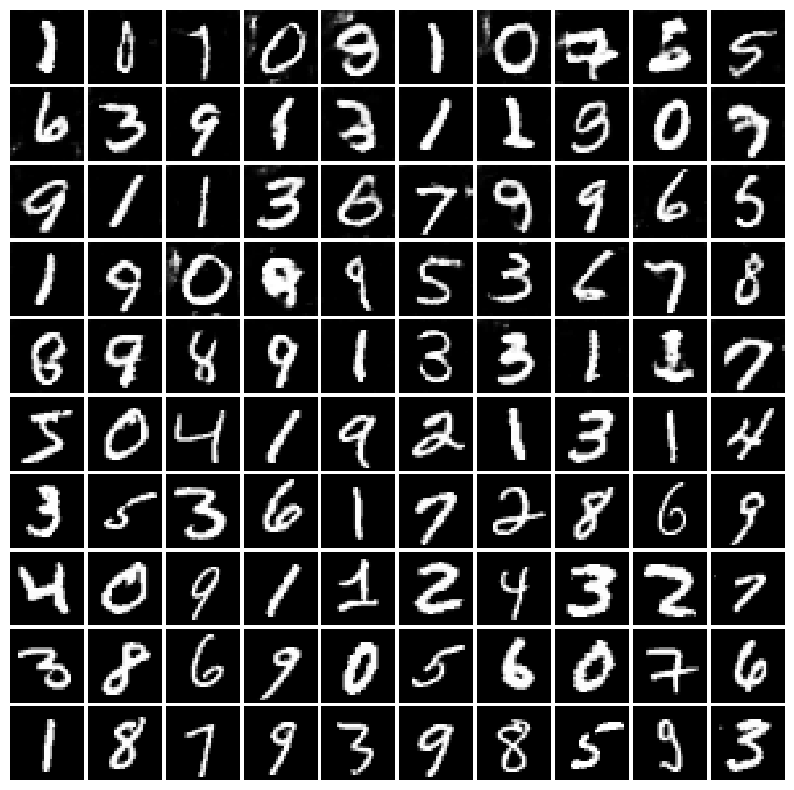
\includegraphics[width=0.85\linewidth]{dc_gan/real_vs_fake.png}
  \caption{DCGAN samples (top five rows) above real MNIST digits (bottom five rows).}
  \label{fig:realfake}
\end{figure}

\subsubsection{Can the generator win on finite samples?}

The game has an equilibrium, and it is a tie. Goodfellow et al.\ show that the optimal discriminator is \(D = 1/2\) everywhere exactly when \(p_g = p_{\mathrm{data}}\), with game value \(-\log 4\). The generator never ``wins'' by making the discriminator wrong; it can only match the data distribution, after which the discriminator's best strategy is to guess. This run does not reach that point even in the loss: the late DCGAN discriminator loss is about \(1.0\)--\(1.1\), not \(1.39\), so the discriminator being trained still separates real from fake on its minibatches.

Reaching chance in the training loss would still not make the two finite samples indistinguishable. A fresh, high-capacity classifier trained to convergence against a frozen generator can exploit any residual difference: speckle, a broken stroke, a small shift in stroke thickness. Making the two empirical distributions identical would require the generator to reproduce the training set, which none of these runs does. Vanilla and LS samples are obvious fakes, and DCGAN samples, though close, are still separable both by the training discriminator and by eye. So the equilibrium exists in theory, but a generator that makes finite samples truly indistinguishable is not something this run reaches, and it is not what one-step alternating updates on finite networks are set up to guarantee.

\newpage
%%%%%%%%%%%%%%%%%%%%%%%%%%%%%%%%%%%%%%%%%%%%%%%%%%%%%%%%%%%%%%%%%%%%%%%%
\section{Problem 2: EBMs on MNIST (40 points)}
%%%%%%%%%%%%%%%%%%%%%%%%%%%%%%%%%%%%%%%%%%%%%%%%%%%%%%%%%%%%%%%%%%%%%%%%

\begin{question}
You will implement an Energy Based Model and evaluate it for generative performance and anomaly detection capacity, using the notebook \texttt{ebm-mnist.ipynb}.
\begin{enumerate}
  \item[(a)] Part 0/1: Libraries and utility functions. How does the contrastive divergence objective change the energy of the correct/wrong samples? What do you think would need to happen for the push/pull forces on the diagram to balance out?
  \item[(b)] Part 2: Model construction and training. Implement the model construction, MCMC sampling steps, and loss calculation, and run the implemented model.
  \begin{itemize}
    \item Why do you think that the Swish activation function is more convenient than the standard ReLU for this model and task? \emph{Hint: visualize both activation functions and think about how they would affect the backward propagation of the gradient through the network.}
    \item What is the role of the regularization loss? How do you think the resulting data would look if we were not using it?
  \end{itemize}
  \item[(c)] Part 3: Analysis. Sample a few images using the MCMC method. How many MCMC steps are required to sample reasonable images from the trained model? Is this number different for different digits? Then complete the transformation cells to test the out-of-distribution performance of the model.
  \begin{itemize}
    \item For pure random noise inputs: are the scores in line with what would be expected for a good anomaly detection method? Why do you think the score for the `true' images is so close to zero?
    \item For the image transformations: do the scores of the transformed images differ significantly from the original ones? Do you think this model would make a good out-of-distribution detector? Provide a detailed explanation of why this would or would not be the case.
  \end{itemize}
\end{enumerate}
\end{question}

The network outputs a scalar score \(f_\theta(x)\), and the notebook defines the model density as
\begin{equation}
  q_\theta(x) = \frac{\exp\bigl(f_\theta(x)\bigr)}{Z_\theta},
  \qquad
  f_\theta(x) = -E_\theta(x),
  \label{eq:ebm-q}
\end{equation}
so a high score means low energy and high unnormalized probability. The normalizer \(Z_\theta\) integrates \(\exp(f_\theta)\) over all images and is intractable. Images are scaled to \([-1,1]\), which is also the box the sampler is clipped to.

\subsection{Part 0/1: Contrastive divergence}

Maximum likelihood minimizes \(\mathcal{L}(\theta) = -\mathbb{E}_{p(x)}[\log q_\theta(x)]\). Since \(\log q_\theta(x) = f_\theta(x) - \log Z_\theta\) and \(\nabla_\theta \log Z_\theta = \mathbb{E}_{q_\theta(x)}[\nabla_\theta f_\theta(x)]\),
\begin{equation}
  \nabla_\theta \mathcal{L}
  = \mathbb{E}_{q_\theta(x)}\bigl[\nabla_\theta f_\theta(x)\bigr]
  - \mathbb{E}_{p(x)}\bigl[\nabla_\theta f_\theta(x)\bigr].
  \label{eq:cd-grad}
\end{equation}
A descent step therefore raises \(f_\theta\) on data and lowers it on model samples. In energy terms, that is the pair of forces in the diagram.

\subsubsection{Effect on the energy of correct and wrong samples}

The ``correct answer'' is a training image \(x_{\mathrm{train}} \sim p(x)\); the update lowers its energy, pulling it down the energy curve and making it more probable. The ``wrong answer'' is a model sample \(x_{\mathrm{sample}} \sim q_\theta(x)\); the update raises its energy and makes it less probable. Replacing the model expectation with one sample gives the contrastive divergence loss used later,
\begin{equation}
  \ell_{\mathrm{CD}} = f_\theta(x_{\mathrm{sample}}) - f_\theta(x_{\mathrm{train}})
  = E_\theta(x_{\mathrm{train}}) - E_\theta(x_{\mathrm{sample}}),
  \label{eq:cd-loss}
\end{equation}
and minimizing it is the same push and pull: down on data, up on samples.

\subsubsection{When the push and pull balance}

The gradient~\eqref{eq:cd-grad} vanishes when \(\mathbb{E}_{p}[\nabla_\theta f_\theta] = \mathbb{E}_{q_\theta}[\nabla_\theta f_\theta]\), which holds once \(q_\theta = p\). Model samples then land on the same images as the training data, so the upward push on ``wrong'' samples and the downward pull on ``correct'' ones act on the same regions and cancel. Until then, mass sitting off the data keeps being pushed up and real digits keep being pulled down.

\subsection{Part 2: Model construction and training}

\subsubsection{Energy network}

\(f_\theta\) is a small CNN with Swish activations, \(x\,\sigma(x)\). On a \(1\times 28\times 28\) image:
\begin{center}
\begin{tabular}{lll}
\toprule
Layer & Shape & Activation \\
\midrule
Conv \(5\times 5\), stride 2, pad 4 & \(1 \to 16\), \(16\times 16\) & Swish \\
Conv \(3\times 3\), stride 2, pad 1 & \(16 \to 32\), \(8\times 8\) & Swish \\
Conv \(3\times 3\), stride 2, pad 1 & \(32 \to 64\), \(4\times 4\) & Swish \\
Conv \(3\times 3\), stride 2, pad 1 & \(64 \to 64\), \(2\times 2\) & Swish \\
Flatten & \(256\) & none \\
Linear & \(256 \to 64\) & Swish \\
Linear & \(64 \to 1\) & none \\
\bottomrule
\end{tabular}
\end{center}
The output is squeezed to one score \(f_\theta(x) = -E_\theta(x)\) per image. The network has \(76{,}993\) parameters.

\subsubsection{Langevin sampler}

Samples come from short-run Langevin dynamics in the box \([-1,1]\). Each of \(K\) steps, with step size \(\nu\), is
\begin{align}
  x &\leftarrow \mathrm{clip}\bigl(x + \omega,\, -1,\, 1\bigr),
  & \omega &\sim \mathcal{N}(0,\, 0.005^{2}), \nonumber \\
  g &\leftarrow \mathrm{clip}\bigl(\nabla_x E_\theta(x),\, -0.03,\, 0.03\bigr), \nonumber \\
  x &\leftarrow \mathrm{clip}\bigl(x - \nu g,\, -1,\, 1\bigr).
  \label{eq:langevin}
\end{align}
The gradient of \(E_\theta = -f_\theta\) is taken with the weights frozen and clipped so a single step cannot jump across the image; \(x - \nu g\) walks downhill in energy. Training uses \(K = 60\) and \(\nu = 10\). The generation plots use \(K = 256\) from fresh noise.

A replay buffer of up to \(8{,}192\) images supplies the starting points: \(95\%\) of each batch comes from the buffer and \(5\%\) from fresh uniform noise, and the new samples go to the front of the buffer. These warm starts are why \(60\) steps suffice during training, since most chains already start near a mode.

\subsubsection{Loss}

Real images get pixel noise with standard deviation \(0.005\) and are clipped back to \([-1,1]\). The network scores the real and sampled batches together, and with \(f_{\mathrm{real}}\), \(f_{\mathrm{fake}}\) those scores,
\begin{align}
  \ell_{\mathrm{CD}} &= \mathbb{E}[f_{\mathrm{fake}}] - \mathbb{E}[f_{\mathrm{real}}], \\
  \ell_{\mathrm{reg}} &= \mathbb{E}\bigl[f_{\mathrm{real}}^{2} + f_{\mathrm{fake}}^{2}\bigr], \\
  \ell &= \ell_{\mathrm{CD}} + \alpha\,\ell_{\mathrm{reg}},
  \qquad \alpha = 0.1.
  \label{eq:ebm-loss}
\end{align}
\(\ell_{\mathrm{CD}}\) is the batch version of~\eqref{eq:cd-loss}. The optimizer is Adam with learning rate \(10^{-4}\) and betas \((0, 0.999)\); first-moment momentum is off because the loss surface moves as the negative samples change. The learning rate decays by \(0.97\) per epoch, and gradients are clipped to global norm \(0.1\). The model was trained for the full \(60\) epochs with batch size \(128\) on a single NVIDIA H100 on PACE ICE. The checkpoint used below is the best one by validation contrastive divergence, from epoch \(58\) (counting from \(0\), so the \(59\)th of \(60\)) at step \(27{,}612\).

\subsubsection{Swish vs.\ ReLU}

Swish is smooth: for positive inputs it approaches \(y = x\), and for negative inputs it dips slightly below zero and returns toward it. Its derivative,
\[
  \sigma(x)\bigl(1 + x\bigl(1-\sigma(x)\bigr)\bigr),
\]
is continuous and is zero only at the single point \(x \approx -1.28\). ReLU's derivative is exactly zero on all of \(x < 0\) and jumps at the origin.

That matters because sampling follows \(\nabla_x f_\theta(x)\), which has to backpropagate through every activation. Wherever a ReLU unit is off, that part of the energy surface is flat, the input gradient dies, and the Langevin chain stalls. Swish still passes a slope through those regions, so both the sampler and the parameter updates keep a direction. ReLU's kink also makes \(\nabla_x f_\theta\) discontinuous, which makes Langevin steps jumpy; Swish keeps \(f_\theta\) smooth.

\subsubsection{Role of the regularization loss}

Contrastive divergence only sees the gap \(f_{\mathrm{fake}} - f_{\mathrm{real}}\). That gap can grow without bound by sending real scores to \(+\infty\) and fake scores to \(-\infty\), which doesn't change which images are relatively likely but turns the energy surface into a cliff. Langevin steps would then always hit the \(\pm 0.03\) gradient cap and slam into the \(\pm 1\) walls, the samples would become saturated noise or harsh blobs, and training would diverge.

The penalty \(\alpha\,\mathbb{E}[f_{\mathrm{real}}^{2} + f_{\mathrm{fake}}^{2}]\) keeps both scores near zero, so training has to shape the surface rather than just stretch it. It is also why real-image scores sit near zero in Part~3: zero is the scale the regularizer picked, not a statement that the probability is \(1\).

\subsection{Part 3: Analysis}

Everything below uses that checkpoint. For the sampling figure, eight chains start from independent uniform noise and run \(256\) steps of~\eqref{eq:langevin} with \(\nu = 10\).

\subsubsection{Image generation and number of MCMC steps}

\begin{figure}[H]
  \centering
  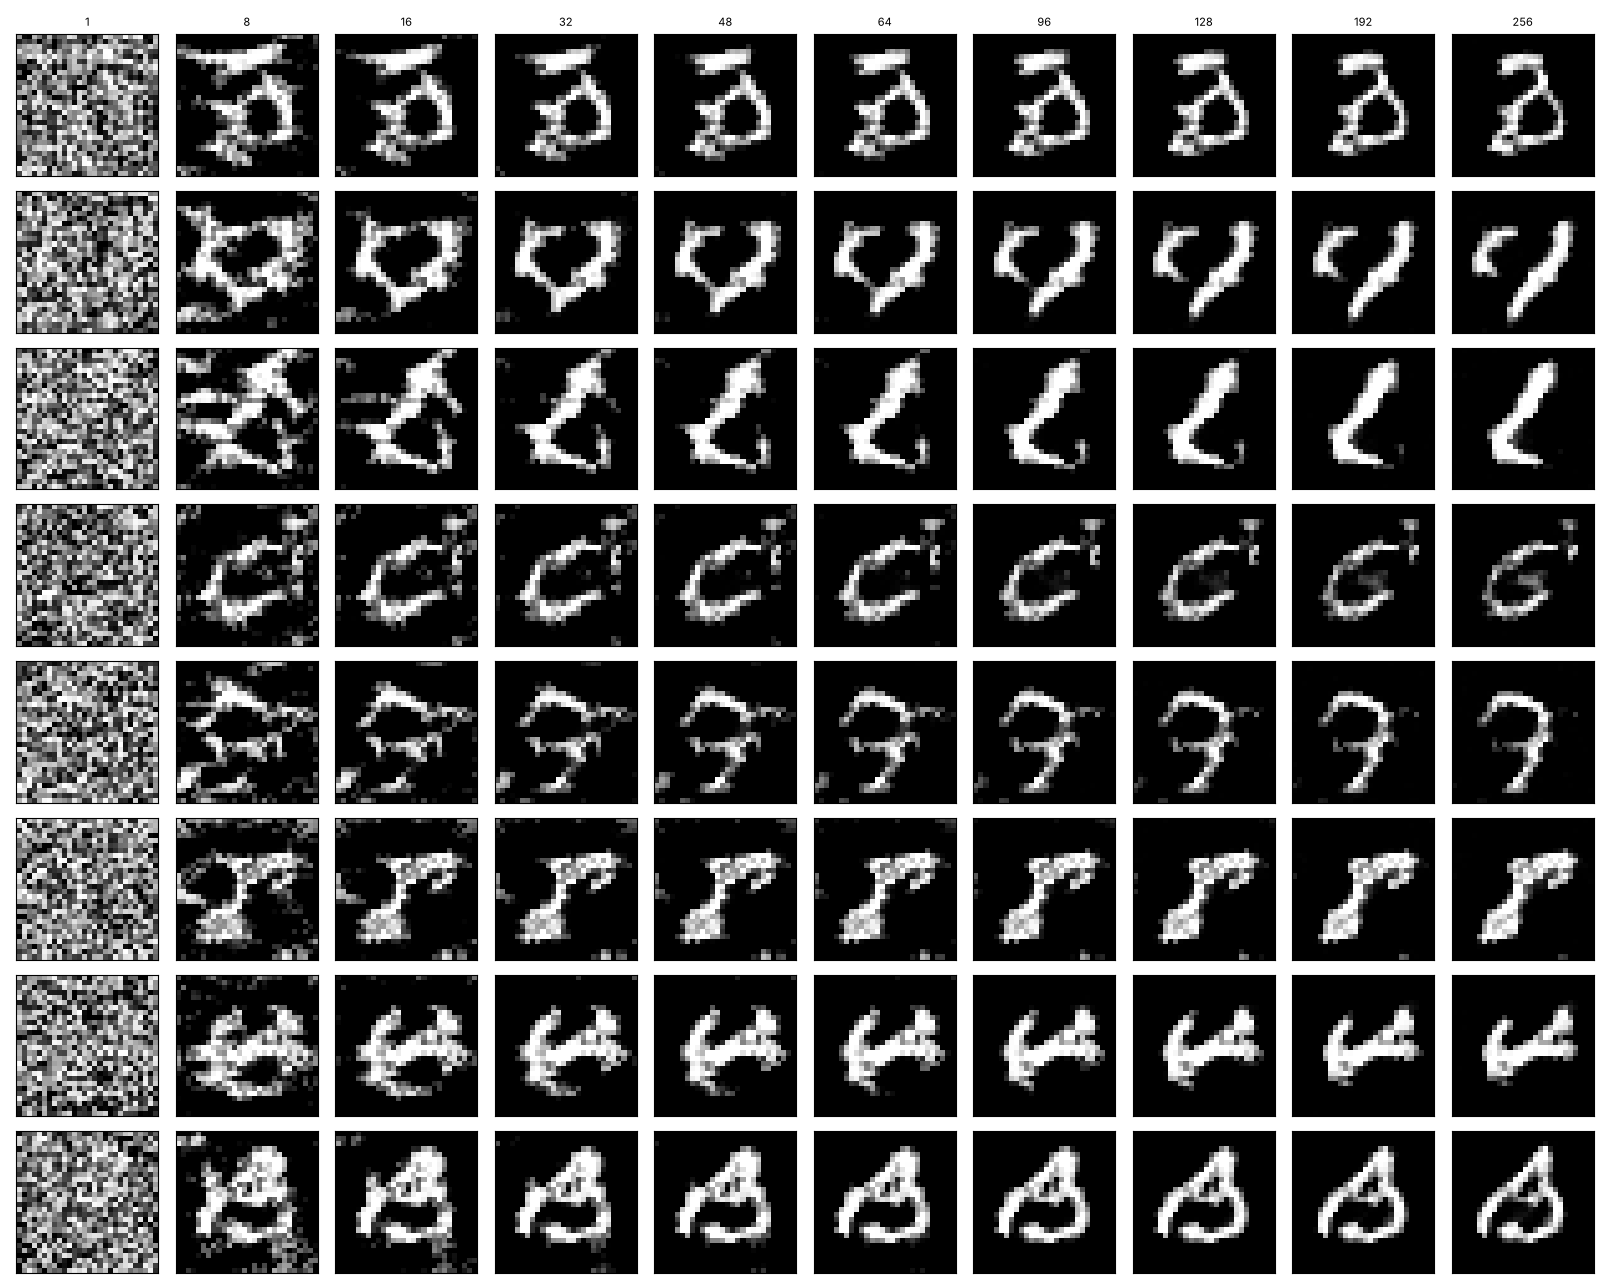
\includegraphics[width=0.95\linewidth]{ebm/mcmc_steps.png}
  \caption{Eight Langevin chains started from uniform noise. Columns are the image after the listed number of steps.}
  \label{fig:ebm-mcmc}
\end{figure}

Step \(1\) is noise. By step \(8\) every chain has a dark background and a bright stroke pattern, and by steps \(32\)--\(48\) most shapes have locked in: the top chain is a \(2\), the third an L-shaped stroke, the fifth a \(7\) with a closed top, and the bottom chain a closed loop. Shapes that have to open or add a stroke take longer. The second chain is a closed V until it opens into a hooked \(7\) around step \(128\), and the fourth is a C until about step \(192\), when it grows an inner stroke and settles toward a \(6\). The sixth and seventh chains are stable by step \(64\) but never become clear digits. Apart from the fourth chain, little changes between steps \(128\) and \(256\) beyond cleaner edges.

So a stable shape takes about \(32\)--\(64\) steps from pure noise, and a recognizable digit, when the chain reaches one, about \(64\)--\(192\). The number depends on the digit: simple strokes and closed loops lock in early, while shapes that need to open or add a stroke keep changing. Only about half of the eight chains end as clear digits, so the model's samples are rougher than its scores on real data suggest. The \(60\) steps used in training are not comparable, because \(95\%\) of those chains start from the replay buffer; from scratch, \(60\) steps only reach the easy shapes.

\subsubsection{Out-of-distribution: random noise}

The score is \(f_\theta\), and lower means less probable. On \(256\) images of each kind:
\begin{center}
\begin{tabular}{lcc}
\toprule
Input & Mean \(f_\theta\) & Spread \\
\midrule
Uniform noise on \([-1,1]\) & \(-15.70\) & all scores in \([-16.11,\,-15.33]\) \\
MNIST test digits & \(0.01\) & std \(0.02\), range \([-0.09,\,0.04]\) \\
MNIST training digits & \(0.00\) & std \(0.03\) \\
\bottomrule
\end{tabular}
\end{center}
A gap of about \(16\) against a real-digit spread of \(0.02\) is exactly what a good anomaly detector should show for unstructured noise.

Real digits sit near zero because of the regularizer in~\eqref{eq:ebm-loss}. The contrastive term only needs \(f(\mathrm{real})\) above \(f(\mathrm{fake})\), and the quadratic penalty is smallest when both are near zero, so the optimizer parks data at about \(0\) and pushes everything else far negative. The score is an unnormalized log-density, so zero just means ``on the scale \(\ell_{\mathrm{reg}}\) chose.''

\subsubsection{Out-of-distribution: image transformations}

The same \(256\) test digits were corrupted three ways: Gaussian noise of scale \(0.3\), clipped to \([-1,1]\); a flip of both spatial axes; and the digit shrunk into the bottom-right corner on a background of \(-1\).
\begin{center}
\begin{tabular}{lc}
\toprule
Transform of the \(256\) test digits & Mean \(f_\theta\) \\
\midrule
Original & \(0.01\) \\
Noise, scale \(0.3\) & \(-0.17\) \\
Flipped vertically and horizontally & \(-0.01\) \\
Shrunk into the corner & \(-0.05\) \\
\bottomrule
\end{tabular}
\end{center}

\begin{figure}[H]
  \centering
  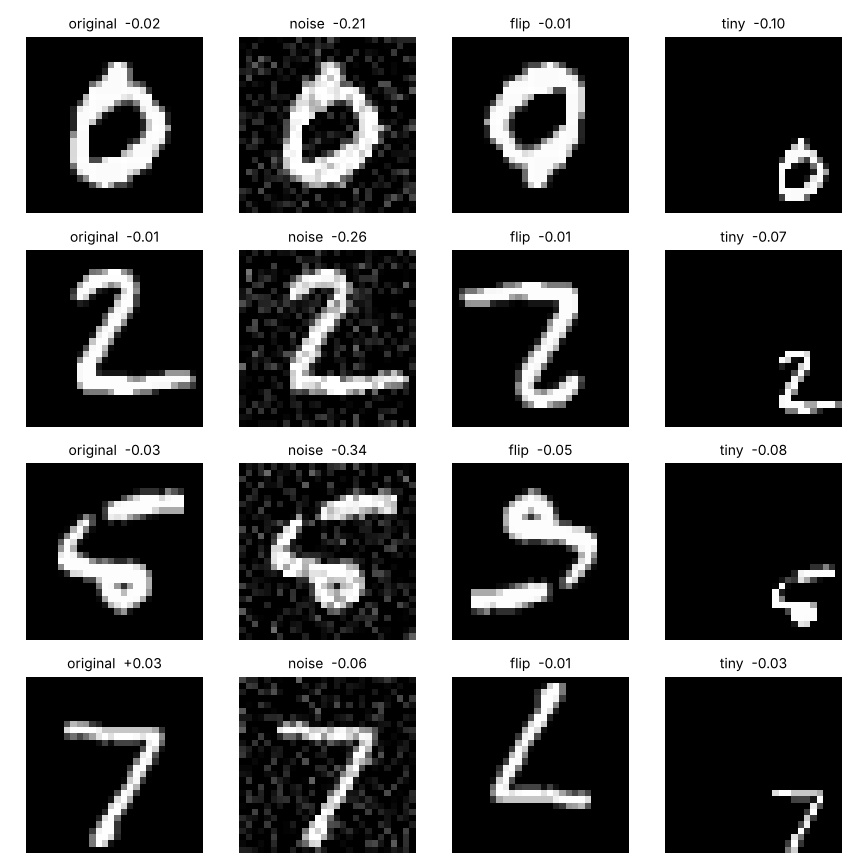
\includegraphics[width=0.62\linewidth]{ebm/transforms.png}
  \caption{Scores \(f_\theta\) for four test digits after the three transformations. Titles are the score of that image.}
  \label{fig:ebm-transforms}
\end{figure}

Noise moves the score by only a few tenths. In Figure~\ref{fig:ebm-transforms} the noisy \(0\) goes from \(-0.02\) to \(-0.21\), the noisy \(5\) from \(-0.03\) to \(-0.34\), and the noisy \(7\) only from \(+0.03\) to \(-0.06\), still inside the range of real scores (the worst test digit in the batch scored \(-0.09\)). Flipped digits are no longer valid instances of their class, yet the batch mean moves by only \(0.02\), and the four flips in the figure by at most \(0.04\). The shrunk digits are the wrong size in the wrong place and move only slightly more: the shrunk \(0\) goes from \(-0.02\) to \(-0.10\), just below the worst real digit, and the shrunk \(7\) from \(+0.03\) to \(-0.03\).

\subsubsection{Is this a good OOD detector?}

It is a good detector of the kind of negatives it was trained against, and a weak detector of anything else.

Unstructured noise sits about \(16\) units below the data with no overlap, so any threshold between \(-1\) and \(-15\) rejects it and keeps ordinary digits. That is what contrastive divergence with short-run Langevin is built for: the negative phase is noise or a short chain that hasn't reached the data yet, so the model learns to score that region low.

Flips and large changes of scale and position are also outside the MNIST generative process, but the scores barely register them. The gap from a real digit to a flipped or shrunk one is a few hundredths, comparable to the spread of real digits (std \(0.02\)), so a threshold that rejected them would also reject ordinary test digits. Pixel noise shifts the mean to \(-0.17\), a real effect, but individual noisy digits still overlap the worst real scores, so the sets are not separable.

The cause is specific. The negative samples never include flipped or rescaled digits, so nothing in~\eqref{eq:cd-grad} raises the energy of an image that still contains plausible local strokes, and the CNN mostly scores those strokes; a flipped \(7\) and a tiny \(2\) both have them. The regularizer then squeezes every in-distribution score toward \(0\), leaving almost no room for a slightly wrong image to stand apart. The model responds to ``stroke on background at roughly the right contrast'' and is insensitive to class identity, orientation, and layout. That is enough to reject pure noise, but not enough for a general out-of-distribution detector.

\newpage
%%%%%%%%%%%%%%%%%%%%%%%%%%%%%%%%%%%%%%%%%%%%%%%%%%%%%%%%%%%%%%%%%%%%%%%%
\section{GDL-Bench Challenge Problem (20 points)}
%%%%%%%%%%%%%%%%%%%%%%%%%%%%%%%%%%%%%%%%%%%%%%%%%%%%%%%%%%%%%%%%%%%%%%%%

\begin{question}
As part of each homework, you will contribute one candidate problem to GDL-Bench, a benchmark for evaluating the reasoning capabilities of current AI systems in generative and geometric deep learning. For this homework, design one original challenge problem related to one or more of the topics covered in this assignment. The problem should require genuine mathematical, conceptual, algorithmic, or implementation-level reasoning, and should not be answerable by simply recalling a definition or looking up a fact.
\begin{enumerate}
  \item[(a)] \textbf{Challenge problem.} Write the exact problem as you would like it to appear in GDL-Bench. It must be original, self-contained, technically well-defined, and unambiguous.
  \item[(b)] \textbf{Gold answer and solution.} Provide the correct final answer together with a concise but complete solution, enough for another student or instructor to independently verify the answer. Whenever possible, design the problem so that the final answer can be objectively checked.
  \item[(c)] \textbf{What does the problem test?} Topic; problem type (derivation, conceptual reasoning, counterexample, numerical, coding/debugging, algorithm design, or other); and the core insight in 1--3 sentences, including why a solver with only superficial knowledge might struggle.
  \item[(d)] \textbf{Test AI systems.} Only after the problem and solution are finalized, give the exact same problem to at least two current AI models, with no extra hints and without the solution. For each model report the name/version, whether the answer was Correct, Partially Correct, or Incorrect, and a 1--3 sentence explanation of any important error. A problem does not need to defeat the models to receive full credit.
\end{enumerate}
Quality bar: original, relevant, self-contained, unambiguous, verifiable, and reasoning-intensive. Grading: relevance and originality (4); technical correctness (6); clarity (4); depth of reasoning (4); complete metadata and AI evaluation (2).
\end{question}

The full, agent-runnable version of this problem (task statement, reference
solution, and automated tests) is in \texttt{gdlbench\_submission/}. The
statement below is the text of \texttt{task/TASK.md}.

\subsection{(a) Challenge problem}

\textbf{Which generator does each GAN objective prefer?}

All logarithms are natural, and all distributions live on the nonnegative
integers. The data distribution \(p\) is uniform on \(\{0,1,2,3\}\). For each
positive integer \(k\), the generator distribution \(q_k\) is uniform on
\(\{0,1,\dots,k-1\}\). Conventions: \(\log 0=-\infty\),
\(0\cdot(\pm\infty)=0\), and an expectation that puts positive probability on
an integrand equal to \(+\infty\) is \(+\infty\).

\medskip\noindent\textbf{Definitions.}
\begin{itemize}
  \item \(\mathrm{JSD}(p,q)=\tfrac12\KL(p\|m)+\tfrac12\KL(q\|m)\), with \(m=(p+q)/2\).
  \item \emph{Minimax GAN.} For a discriminator \(D\) mapping integers to \([0,1]\),
  \[
    V(D,q)=\E_{x\sim p}[\log D(x)]+\E_{x\sim q}[\log(1-D(x))].
  \]
  Let \(D^*_q\) maximize \(V(D,q)\) (its values off the support of \(p+q\) do
  not matter), and define
  \[
    V_\star(q)=V(D^*_q,q),\qquad
    L_{\mathrm{MM}}(q)=\E_{x\sim q}[\log(1-D^*_q(x))],\qquad
    L_{\mathrm{NS}}(q)=\E_{x\sim q}[-\log D^*_q(x)].
  \]
  \item \emph{Least-squares GAN} with labels \(a=-1\) (generated), \(b=1\)
  (real), and generator target \(c=0\). The discriminator \(D^{\mathrm{LS}}_q\)
  minimizes \(\tfrac12\E_p[(D-1)^2]+\tfrac12\E_q[(D+1)^2]\) over real-valued
  \(D\), and the generator criterion is
  \[
    V_{\mathrm{LS}}(q)=\tfrac12\E_{x\sim p}\bigl[(D^{\mathrm{LS}}_q(x)-0)^2\bigr]
    +\tfrac12\E_{x\sim q}\bigl[(D^{\mathrm{LS}}_q(x)-0)^2\bigr].
  \]
\end{itemize}
The generator wants each of \(V_\star\), \(L_{\mathrm{MM}}\),
\(L_{\mathrm{NS}}\), and \(V_{\mathrm{LS}}\) to be as small as possible.

\medskip\noindent\textbf{Report:}
\begin{enumerate}
  \item \texttt{jsd\_tie\_pairs}: every unordered pair \(\{j,k\}\) of distinct
        positive integers with \(\mathrm{JSD}(p,q_j)=\mathrm{JSD}(p,q_k)\) exactly.
  \item \texttt{ls\_tie\_pairs}: every unordered pair \(\{j,k\}\) of distinct
        positive integers with \(V_{\mathrm{LS}}(q_j)=V_{\mathrm{LS}}(q_k)\) exactly.
  \item \texttt{ls\_value\_q2}: the value of \(V_{\mathrm{LS}}(q_2)\).
  \item \texttt{k\_hat}: the integer \(\hat k\neq2\) such that \(\{2,\hat k\}\)
        is in \texttt{jsd\_tie\_pairs}, or \texttt{null} if there is none.
  \item If \(\hat k\) exists: the values of \(V_\star\), \(L_{\mathrm{MM}}\),
        and \(L_{\mathrm{NS}}\) at \(q_2\) and at \(q_{\hat k}\).
  \item If \(\hat k\) exists: for each of \(V_\star\), \(L_{\mathrm{MM}}\),
        \(L_{\mathrm{NS}}\), which of \(q_2\) and \(q_{\hat k}\) the generator
        prefers (lower value), or \texttt{"tie"}.
\end{enumerate}
The solver also writes a short derivation that justifies why the lists in
items 1 and 2 are \emph{complete}. Answers go in
\texttt{task/results/answer.json}, with \(+\infty\) written as the string
\texttt{"inf"} and floats to at least 10 significant figures. Pair lists,
\(\hat k\), \texttt{"inf"}, and preferences must match exactly; floats must be
within \(10^{-8}\).

\subsection{(b) Gold answer and solution}

\begin{center}
\begin{tabular}{@{}lll@{}}
\toprule
Key & Gold answer & Value\\
\midrule
\texttt{jsd\_tie\_pairs} & \(\{1,16\},\ \{2,8\}\) & \\
\texttt{ls\_tie\_pairs} & \(\{1,16\},\ \{2,8\}\) & \\
\texttt{ls\_value\_q2} & \(1/3\) & \(0.333333\)\\
\texttt{k\_hat} & \(8\) & \\
\(V_\star(q_2)=V_\star(q_8)\) & \(\log2-\tfrac32\log3\) & \(-0.954771\)\\
\(L_{\mathrm{MM}}(q_2)\) & \(\log(2/3)\) & \(-0.405465\)\\
\(L_{\mathrm{MM}}(q_8)\) & \(-\tfrac12\log3\) & \(-0.549306\)\\
\(L_{\mathrm{NS}}(q_2)\) & \(\log3\) & \(1.098612\)\\
\(L_{\mathrm{NS}}(q_8)\) & \(+\infty\) & \\
\texttt{prefers} & \multicolumn{2}{l}{\(V_\star\): tie;\quad \(L_{\mathrm{MM}}\): \(q_8\);\quad \(L_{\mathrm{NS}}\): \(q_2\)}\\
\bottomrule
\end{tabular}
\end{center}

\paragraph{Both criteria depend only on a support ratio.} The distributions
\(p\) and \(q_k\) are nested uniforms. Let the smaller one have support size
\(n\) and the larger one \(N\), and let \(r=N/n=\max(k,4)/\min(k,4)\ge1\). On
the shared support \(m=(r+1)/(2N)\); off it, \(m=1/(2N)\). Then
\[
  \KL(\text{small}\|m)=\log\frac{2r}{r+1},\qquad
  \KL(\text{large}\|m)=\frac1r\log\frac{2}{r+1}+\Bigl(1-\frac1r\Bigr)\log2,
\]
so
\[
  \mathrm{JSD}(r)=\log2+\tfrac12\log r-\tfrac12\Bigl(1+\tfrac1r\Bigr)\log(1+r),
  \qquad
  \frac{d\,\mathrm{JSD}}{dr}=\frac{\log(1+r)}{2r^2}>0 .
\]
JSD is symmetric, so it does not matter which of \(p\) and \(q_k\) is the
larger one. JSD is therefore a strictly increasing function of \(r\) alone,
and \(\mathrm{JSD}(p,q_j)=\mathrm{JSD}(p,q_k)\) holds iff \(r_j=r_k\). For
\(j\neq k\) this needs one index below 4 and one above it, with \(4/j=k/4\),
i.e.\ \(jk=16\). The only integer solutions are \(\{1,16\}\) and \(\{2,8\}\)
(\(j=3\) gives \(16/3\)). The argument covers every positive integer, so the
list is complete, and \(\hat k=8\).

\paragraph{LSGAN.} Minimizing \(\tfrac12p(D-1)^2+\tfrac12q(D+1)^2\) pointwise
gives \(D^{\mathrm{LS}}=(p-q)/(p+q)\). Substituting,
\[
  V_{\mathrm{LS}}=\frac12\sum_x\frac{(p-q)^2}{p+q}
  =\frac12\Bigl[\frac{(r-1)^2}{r(r+1)}+\frac{r-1}{r}\Bigr]
  =\frac{r-1}{r+1},
\]
which is also strictly increasing in \(r\) alone. The tie pairs are the same,
and \(V_{\mathrm{LS}}(q_2)=1/3\).

\paragraph{Why the ties happen.} An \(f\)-divergence depends only on the
distribution of the likelihood ratio \(p/q\). The pair \((p,q_2)\) has the
same ratio structure as \((q_8,p)\): a uniform against a uniform on half its
support. Hence \(D_f(p\|q_2)=D_g(p\|q_8)\) with the reversed generator
\(g(u)=u\,f(1/u)\). Every symmetric \(f\)-divergence (JSD, the LSGAN
\(\chi^2\)-type term) must tie on this pair. Only asymmetric ones can tell
mode dropping (\(q_2\)) apart from over-spreading (\(q_8\)).

\paragraph{GAN terms.} \(D^*=p/(p+q)\).
\begin{itemize}
  \item \(q_2\): \(D^*=1/3\) on \(\{0,1\}\), \(D^*=1\) on \(\{2,3\}\).
  Then \(V_\star=\tfrac12\log\tfrac13+\log\tfrac23=\log2-\tfrac32\log3\),
  \(L_{\mathrm{MM}}=\log\tfrac23\), and \(L_{\mathrm{NS}}=\log3\).
  \item \(q_8\): \(D^*=2/3\) on \(\{0,\dots,3\}\), \(D^*=0\) on \(\{4,\dots,7\}\).
  Then \(V_\star=\log\tfrac23+\tfrac12\log\tfrac13+\tfrac12\log1=\log2-\tfrac32\log3\),
  \(L_{\mathrm{MM}}=\tfrac12\log\tfrac13=-\tfrac12\log3\), and
  \(L_{\mathrm{NS}}=\tfrac12\log\tfrac32+\tfrac12(+\infty)=+\infty\).
\end{itemize}
\(V_\star=2\,\mathrm{JSD}-\log4\) ties, as it must. The generator's own minimax
term does \emph{not} tie: the \(\E_p[\log D^*]\) term also depends on \(q\)
through \(D^*\), and dropping it leaves a quantity that favors \(q_8\). The
non-saturating loss is infinite for any generator that puts mass where the
data has none, so it favors \(q_2\), the generator that drops modes. The same
game value gives three different verdicts.

\paragraph{Verification.} \texttt{gt\_code/reference\_solution.py} evaluates
every quantity directly from the distributions (exact fractions wherever no
logarithm is involved), scans \(k=1,\dots,512\) for ties, and asserts
agreement with the closed forms and with \(V_\star=2\,\mathrm{JSD}-\log4\).
\texttt{tests/test\_solution.py} passes 8/8 on the gold answer, and each of
the following mistakes fails at least one test:
\begin{center}
\begin{tabular}{@{}ll@{}}
\toprule
Mistake & Fails\\
\midrule
Report only \(\{2,8\}\) (miss the pair below 4) & \texttt{test\_jsd\_tie\_pairs}\\
Treat \(L_{\mathrm{MM}}\) like \(V_\star\) (claim it ties) & \texttt{test\_q\_k\_hat\_terms}, \texttt{test\_prefers}\\
Assume non-saturating has the same optimum (``tie'') & \texttt{test\_prefers}\\
Drop the \(\tfrac12\) in \(V_{\mathrm{LS}}\) (report \(2/3\)) & \texttt{test\_ls\_value\_q2}\\
Finite \(L_{\mathrm{NS}}(q_8)\) (ignore \(D^*=0\) off the data support) & \texttt{test\_q\_k\_hat\_terms}\\
\bottomrule
\end{tabular}
\end{center}

\subsection{(c) What does the problem test?}

\begin{itemize}
  \item \textbf{Topic:} GAN objectives and the divergences they minimize
        (minimax/JSD, non-saturating loss, LSGAN/Pearson-type \(\chi^2\)),
        mode dropping vs.\ mode covering.
  \item \textbf{Problem type:} derivation, conceptual reasoning, and
        counterexample.
  \item \textbf{Core insight:} symmetric \(f\)-divergences such as JSD and
        the LSGAN criterion depend only on the support ratio, so they cannot
        distinguish dropping half the modes from spreading over twice the
        support; the map \(k\mapsto16/k\) produces exactly the ties. A solver
        with only surface knowledge repeats that ``GANs penalize mode
        collapse'' and treats the game value, the minimax generator term, and
        the non-saturating loss as interchangeable, when in fact they give
        three different preferences on the same pair.
\end{itemize}

\subsection{(d) Testing AI systems}

Each model ran as a coding agent in Cursor, given only \texttt{task/} in a
fresh workspace and the same fixed prompt (no hints, no internet lookup of
the problem, no access to tests or solutions). Each \texttt{answer.json} was
graded with \texttt{tests/test\_solution.py}.

\begin{center}
\begin{tabular}{@{}lll@{}}
\toprule
Model (version) & Result & Tests passed\\
\midrule
Claude Opus 5.5 & Correct & 8/8\\
GPT-5.6-sol & Correct & 8/8\\
Grok 4.7 & Correct & 8/8\\
\bottomrule
\end{tabular}
\end{center}

\begin{itemize}
  \item \textbf{Claude Opus 5.5:} correct. It showed both criteria depend only
        on the support ratio and are monotone in it, which reduces ties to
        \(jk=16\). It also noted \(V_\star=2\,\mathrm{JSD}-\log4\) and
        cross-checked by scanning \(k\le400\) with exact fractions.
  \item \textbf{GPT-5.6-sol:} correct. It gave the same reduction to
        \(u=\min(k/4,4/k)\) with an explicit derivative, and the cleanest
        written derivation of the three.
  \item \textbf{Grok 4.7:} correct, and the most thorough. It derived
        separate closed forms on each side of \(k=4\), proved the identity
        \(\varphi(16/j)=\mathrm{JSD}(p,q_j)\) explicitly, and compared
        values exactly over \(k\le16\).
\end{itemize}
All three found the \(\{1,16\}\) pair, proved the tie lists complete, and
separated \(V_\star\), \(L_{\mathrm{MM}}\), and \(L_{\mathrm{NS}}\) correctly.
None fell into the anticipated traps. Current agentic models with code
execution handle closed-form divergence calculations reliably, so this
problem works best as a clean, verifiable check of the symmetric-divergence
insight and of the difference between the three generator objectives, rather
than as an item that breaks models.


\end{document}
